% \chapter{Second Experimental Evaluation Cycle}

% \section{Design Science Research Framework}

% \section{Context and Problem Statement}

%     \subsection{Context}

%     \subsection{Problem}

% \section{Proposed Artifacts}

% \section{Evaluation}

% 	\subsection{Evaluation Methodology}

% 	\subsection{Data Set Creation}

% 	\subsection{Evaluation Metrics}

%     \subsection{Results}

%     \subsection{Discussion}


\chapter{Second Experimental Evaluation Cycle}
\label{chap:second_experiment}

This chapter describes the second experimental cycle of this research, building upon the findings of the first cycle detailed in Chapter 3. The rapid evolution of generative AI frameworks and models, along with the insights gained previously, prompted a more advanced and rigorous evaluation. This second phase employs non-agentic workflows as a baseline, introduces a more quantitative evaluation methodology, and leverages an automated assessment process based on the "LLM-as-judge" concept \citep{Gu2025}.

The use of "LLM-as-a-judge" was driven by the sheer volume of responses requiring evaluation. With four configurations, two models, and three executions for each of the 33 [AJUSTAR] questions, a total of 792 [AJUSTAR] responses were generated. Manually assessing this volume of data would have been impractical. Furthermore, previously used metrics like `truthfulness` had become less critical. This metric was highly relevant when models frequently hallucinated, a problem that is far less prevalent in the current generation of LLMs, shifting the focus to precision and recall of factual information.

[TODO: GERAR BPMN!!]

\section{Design Science Research Framework}

    This second experimental cycle adheres to the Design Science Research (DSR) methodology, focusing on refining the artifacts and evaluation based on the outcomes of the first cycle.

    \begin{description}
        \item[Context] The operational environment of well construction engineering, where practitioners require efficient and reliable access to vast amounts of technical and ESG-related information.

        \item[Problem] The first experimental cycle revealed several limitations, including the subjective nature and scalability issues of expert-based evaluation, the need to compare agentic systems against simpler non-agentic baselines, and the challenge of ensuring consistent performance. This second cycle addresses the problem of developing a more robust, scalable, and objective method for evaluating and comparing different LLM-based architectures for domain-specific Q\&A.

        \item[Proposed Artifacts] Four distinct architectures were designed and implemented to compare different strategies for information retrieval and reasoning:
        \begin{itemize}
            \item A non-agentic \textbf{Linear-Flow} RAG pipeline.
            \item A non-agentic \textbf{Linear-Flow with a Router} to direct queries.
            \item A \textbf{Single-Agent} architecture, refined from the first experiment.
            \item A \textbf{Multi-Agent Supervisor} architecture for distributed reasoning.
        \end{itemize}

        \item[Evaluation] The artifacts are evaluated using an automated pipeline. An "LLM-as-a-judge" assesses the generated answers against a ground-truth dataset. The evaluation is based on quantitative information retrieval metrics: \textbf{Precision}, \textbf{Recall}, and \textbf{F1-Score}.
    \end{description}

\section{Context and Problem Statement}

    \subsection{Context}

    As established in the previous chapters, this research is situated within the oil and gas industry, specifically in the domain of well construction and maintenance. Engineers and specialists in this field must navigate a complex information landscape, drawing from operational reports, ESG alerts, and documented best practices (Learned Lessons) to make critical decisions. The effectiveness of these decisions hinges on the speed and accuracy with which relevant information can be retrieved and synthesized.

    \subsection{Problem}

    The first experimental cycle confirmed the potential of LLM-based agents but also highlighted key challenges. The manual, expert-led evaluation process was time-consuming and difficult to scale. Furthermore, the performance differences between single and multi-agent systems suggested that a more granular analysis was needed, including a comparison with non-agentic RAG workflows to establish a performance baseline. Therefore, the central problem for this second cycle is to design and execute a more rigorous, automated, and scalable evaluation to definitively compare the efficacy of various agentic and non-agentic architectures in this specialized domain.

% \section{Proposed Artifacts}

%     To address the research problem, four distinct artifacts were developed using the LangChain and LangGraph frameworks. These architectures represent a spectrum of complexity, from simple sequential pipelines to collaborative multi-agent systems.

\section{Proposed Artifacts}

    To address the research problem, four distinct artifacts were developed, representing a spectrum of complexity from simple sequential pipelines to collaborative multi-agent systems. 
    
    \subsection{System Architecture Overview}

    The experimental system was implemented using \citet{Langchain2025} and \citet{Langgraph2025} frameworks specialized in language model orchestration. This modular design allows for the systematic and reproducible evaluation of different components and workflows. Key layers of the architecture include:

    \begin{itemize}
        \item \textbf{Experiment Orchestration:} Manages the execution loop, iterating through all combinations of questions, models, and setups.
        \item \textbf{Agent Workflow Frameworks:} Defines the logic for each of the four proposed artifacts using LangGraph to create cyclical graphs for agentic behavior.
        \item \textbf{Tool Integration:} A standardized interface providing agents with access to external knowledge sources. This layer enables consistent semantic search over domain-specific vector stores, ensuring that performance differences are attributable to architectural choices rather than variations in data access.
        \item \textbf{Prompt Engineering:} A library of system messages and prompt templates designed to guide the LLM's reasoning process for each specific task within the workflows.
        \item \textbf{State Management and Logging:} Captures the complete execution trace of each run, including intermediate steps, tool calls, and final outputs. This observability is essential for understanding not just the final output, but the process by which each architecture arrived at its answer.
    \end{itemize}


    % \subsection{Artifact 1: Linear-Flow}

    %     The Linear-Flow architecture represents the simplest RAG design, where user input is processed in a strictly sequential manner, as shown in Figure \ref{fig:diagrama_linear_flow}. In this setup, a single LLM call handles the generation of search queries for all available tools. The prompts for each tool are concatenated, creating a large and complex context for the LLM. While straightforward, this can lead to performance degradation as the context length increases.

    %     \begin{figure}[h]
    %         \centering
    %         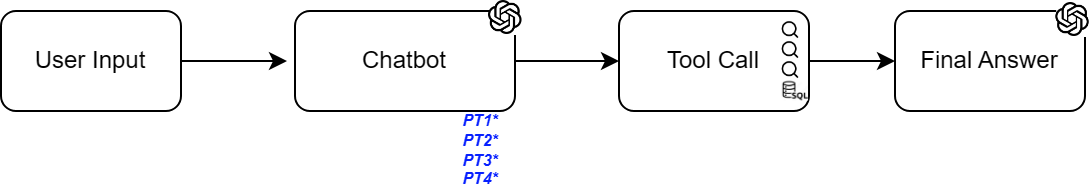
\includegraphics[width=0.8\textwidth]{images_exp2/diagrams/diagrama_linear_flow.png}
    %         \caption{Linear-Flow architecture. PTn indicates the prompt for Tool n.}
    %         \label{fig:diagrama_linear_flow}
    %     \end{figure}

    \subsection{Artifact 1: Linear-Flow}

        The \textbf{Linear-Flow} architecture represents the simplest non-agentic RAG design, serving as a performance baseline. As shown in Figure \ref{fig:diagrama_linear_flow}, user input is processed in a strictly sequential manner. The user's query is handled by a single LLM step, which contains all the instructions needed to generate search queries for every available tool.
        
        \begin{figure}[h]
            \centering
            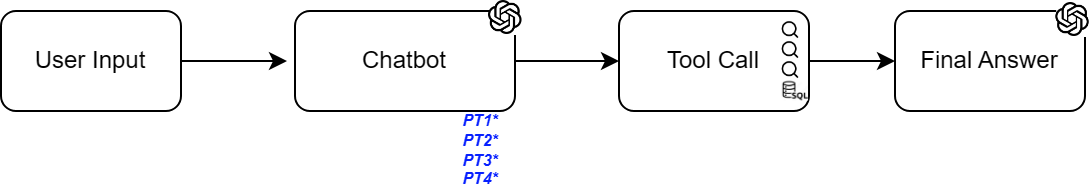
\includegraphics[width=0.8\textwidth]{images_exp2/diagrams/diagrama_linear_flow.png}
            \caption{Linear-Flow architecture. PTn indicates the prompt for Tool n.}
            \label{fig:diagrama_linear_flow}
        \end{figure}

        Because the instruction prompts for all tools are aggregated into a single call, the resulting context for the LLM becomes notably extensive and complex. While this approach is straightforward to implement, its primary drawback is the potential for performance degradation as the context length increases, which can dilute the model's focus and lead to less precise retrieval queries.
        

    % \subsection{Artifact 2: Linear-Flow with Router}
        
    %     This architecture (Figure \ref{fig:diagrama_linear_w_router}) introduces a routing mechanism to improve upon the basic linear flow. A preliminary LLM call acts as a "router," analyzing the user's question and directing it to the most appropriate tool or sequence of tools. This allows for smaller, more specialized prompts for each tool, reducing context length and potentially improving the quality of the generated search queries.

    %     \begin{figure}[h]
    %         \centering
    %         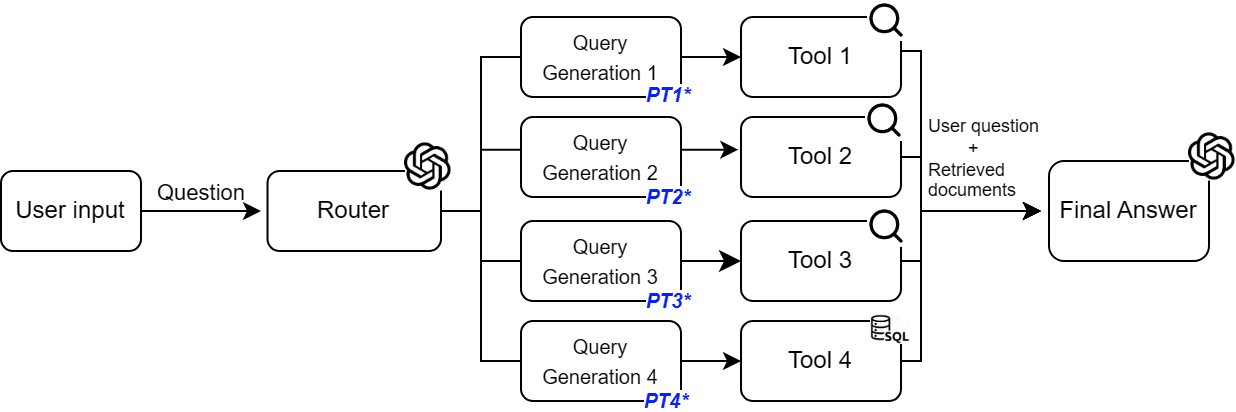
\includegraphics[width=0.8\textwidth]{images_exp2/diagrams/diagrama_linear_w_router.png}
    %         \caption{Linear-Flow with Router architecture.}
    %         \label{fig:diagrama_linear_w_router}
    %     \end{figure}


    \subsection{Artifact 2: Linear-Flow with Router}
    
        The \textbf{Linear-Flow with Router} paradigm (Figure \ref{fig:diagrama_linear_w_router}) extends the basic pipeline by introducing a routing mechanism to create a descentralized, non-agentic workflow. This architecture first directs a user's question to a "router" node, which is a preliminary LLM call tasked with analyzing the query and determining the most appropriate tool or sequence of tools to use.

        \begin{figure}[h]
            \centering
            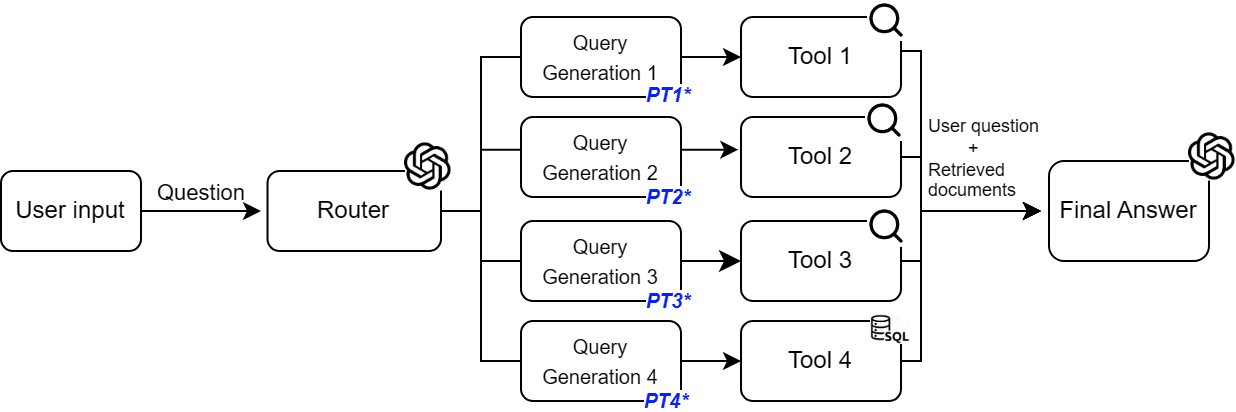
\includegraphics[width=0.8\textwidth]{images_exp2/diagrams/diagrama_linear_w_router.png}
            \caption{Linear-Flow with Router architecture.}
            \label{fig:diagrama_linear_w_router}
        \end{figure}

        This design enables the distribution of complex instruction prompts into smaller, more specialized nodes. Instead of one large prompt, several targeted sub-queries are generated, each dispatched to its respective tool. This approach offers two main advantages:

        \begin{itemize}
            \item \textbf{Specialization:} Each tool receives a query tailored to its specific function, leading to more accurate and relevant retrieval results.
            \item \textbf{Reduced Context:} By breaking down the master prompt, each LLM call operates on a smaller, more focused context, mitigating performance issues associated with long context windows.
        \end{itemize}


    % \subsection{Artifact 3: Single-Agent}

    %     The Single-Agent architecture (Figure \ref{fig:diagrama_single_agent}) represents a centralized agentic approach. A single LLM agent manages the entire question-answering process, autonomously deciding which tools to use, in what order, and how to synthesize the information. This artifact tests the end-to-end reasoning capabilities of an LLM within a unified context, allowing it to perform multi-step reasoning without the overhead of inter-agent communication.

    %     \begin{figure}[h]
    %         \centering
    %         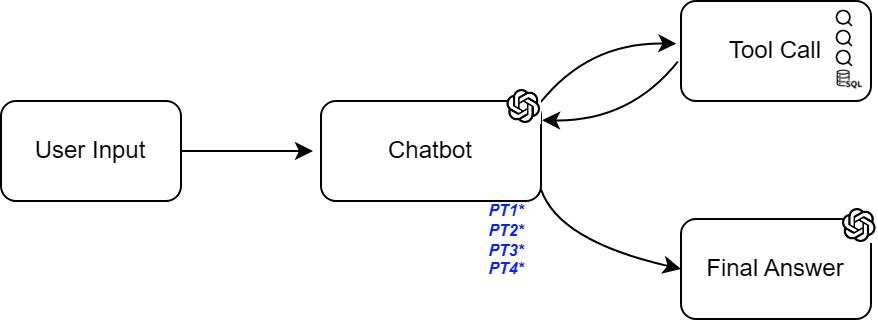
\includegraphics[width=0.5\textwidth]{images_exp2/diagrams/diagrama_single_agent.png}
    %         \caption{Single-Agent architecture.}
    %         \label{fig:diagrama_single_agent}
    %     \end{figure}
    \subsection{Artifact 3: Single-Agent}

        The \textbf{Single-Agent} architecture (Figure \ref{fig:diagrama_single_agent}) embodies a centralized agentic approach, building on the lessons from the first experimental cycle. In this setup, a single LLM agent manages the entire question-answering process. It has access to the full suite of tools and autonomously makes decisions about which to invoke, in what order, and how to synthesize the retrieved information into a final answer.
        
        \begin{figure}[h]
            \centering
            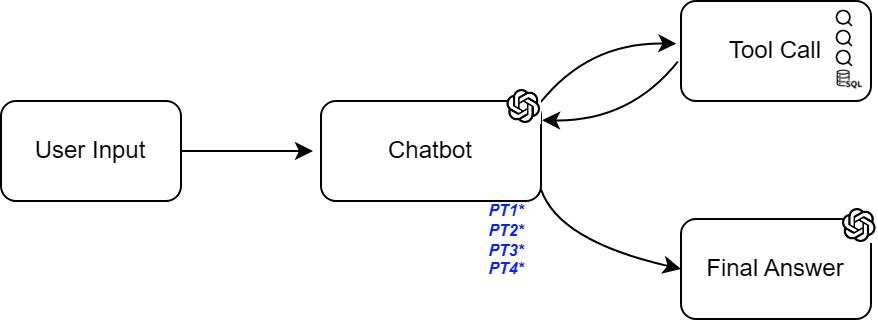
\includegraphics[width=0.5\textwidth]{images_exp2/diagrams/diagrama_single_agent.png}
            \caption{Single-Agent architecture.}
            \label{fig:diagrama_single_agent}
        \end{figure}    

        The design emphasizes \textbf{end-to-end reasoning within a unified context}, allowing the model to maintain the same "thought process" from start to finish. This artifact tests the capability of a standalone LLM agent to manage a RAG workflow, balancing the tool calling for different knowledge sources, all without the communication overhead required by multi-agent systems.
        
    
    % \subsection{Artifact 4: Multi-Agent Supervisor}
        
    %     This setup (Figure \ref{fig:diagrama_multiagente_supervisor}) implements a collaborative, hierarchical agent system. A "supervisor" agent decomposes the user's query and delegates sub-tasks to a team of specialized agents, each with access to a specific tool (e.g., a "Knowledge Items Agent," "ESG Alert Agent"). The supervisor then integrates the findings from the specialists to generate a final, comprehensive answer. This architecture explores the benefits of distributed cognition and task specialization.

    %     \begin{figure}[h]
    %         \centering
    %         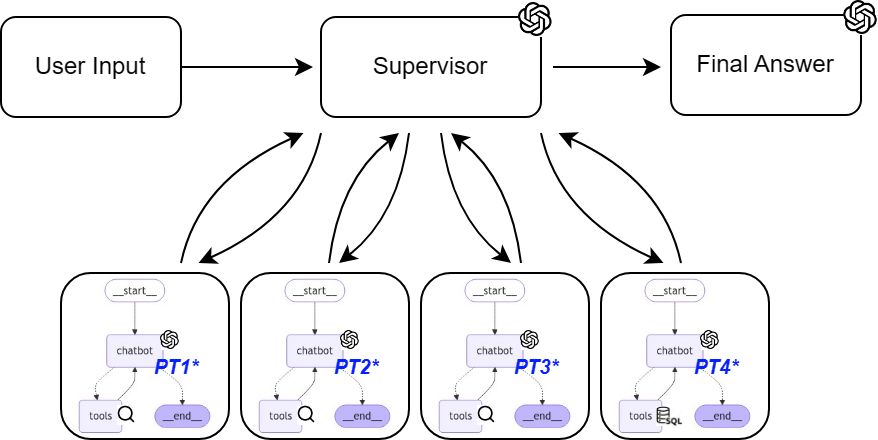
\includegraphics[width=0.6\textwidth]{images_exp2/diagrams/diagrama_multiagente_supervisor.png}
    %         \caption{Multi-Agent Supervisor architecture with four specialist agents.}
    %         \label{fig:diagrama_multiagente_supervisor}
    %     \end{figure}

    \subsection{Artifact 4: Multi-Agent Supervisor}
    
        The \textbf{Multi-Agent Supervisor} setup (Figure \ref{fig:diagrama_multiagente_supervisor}) implements a collaborative, hierarchical system to explore the benefits of distributed cognition. This architecture consists of two main components:        

        \begin{enumerate}
            \item \textbf{A Supervisor Agent:} This master agent receives the user's query, analyzes it, and orchestrates the workflow by delegating these tasks to the appropriate specialist agents.
            \item \textbf{Specialist Agents:} A team of agents, each focusing on a specific domain of knowledge or reasoning skill. For this experiment, each specialist was tied to a single tool (e.g., a "Learned Lessons Agent," an "HSE Alert Agent").
        \end{enumerate}
        
        \begin{figure}[h]
            \centering
            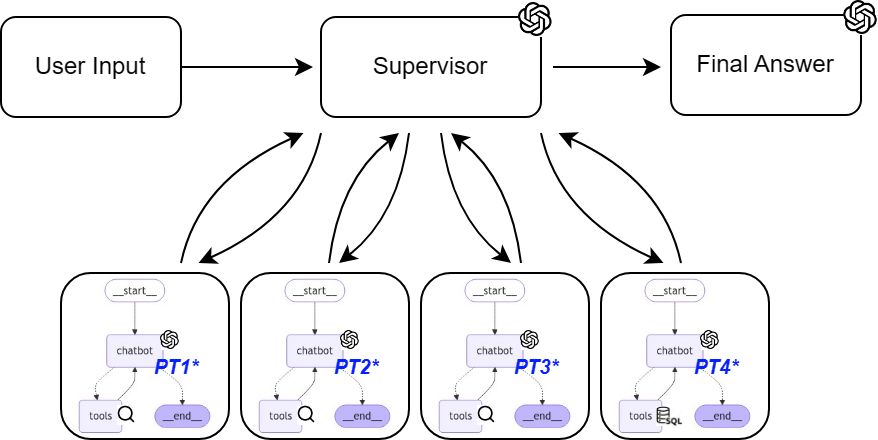
\includegraphics[width=0.6\textwidth]{images_exp2/diagrams/diagrama_multiagente_supervisor.png}
            \caption{Multi-Agent Supervisor architecture with four specialist agents.}
            \label{fig:diagrama_multiagente_supervisor}
        \end{figure}

        The supervisor orchestrates the collaboration, integrates the findings from each specialist, and synthesizes the potentially divergent information into a single, coherent final answer. This framework is designed to mimic real-world expert collaboration and tests whether decomposing a problem and assigning its parts to dedicated specialists yields a more accurate result.
        
        
\section{Evaluation}

    The evaluation phase was designed to be automated, scalable, and objective, addressing the limitations of the first experimental cycle.

    \subsection{Evaluation Methodology}

        The core of the evaluation is an automated execution loop (detailed in Algorithm \ref{alg:execution_loop}) that runs each of the 33 questions through every combination of artifact (4 setups) and model (2 models), repeating each run three times to account for stochasticity.

        \begin{algorithm}[h]
        \caption{Experiment Execution Loop}
        \begin{algorithmic}[1]
        \Require questions, setups, models
        \Ensure results
        \Function{RunExperiment}{}
            \State $results \gets \{\}$
            \ForAll{$question \in questions$}
                \State $ground\_truth \gets question.ground\_truth$
                \ForAll{$setup \in setups$}
                    \ForAll{$model \in models$}
                        \For{$i \in 1 \dots 3$} \Comment{Execute 3 times for consistency}
                            \State $agent \gets \text{InitializeAgent}(setup, model)$
                            \State $response \gets agent.\text{ProcessQuestion}(question)$
                            \State $metrics \gets \text{EvaluateResponse}(response, ground\_truth)$
                            \State Store $metrics$ and $response$ in $results$
                        \EndFor
                    \EndFor
                \EndFor
            \EndFor
            \State \Return $\text{AggregateResults}(results)$
        \EndFunction
        \end{algorithmic}
        \label{alg:execution_loop}
        \end{algorithm}

        The quality of each generated response is assessed using the \textbf{LLM-as-a-Judge} approach. A powerful LLM (GPT-4) is prompted to act as an impartial evaluator, comparing the generated answer against the ground-truth answer. The judge decomposes both texts into atomic statements and classifies them to build a confusion matrix, from which the final metrics are calculated. The full prompt for the LLM-as-a-Judge can be found in Appendix \ref{code:llm-judge}.

    \subsection{Data Set Creation}

        The experiment utilizes a curated dataset developed in collaboration with domain experts.
        \begin{itemize}
            \item \textbf{Questions Dataset:} A set of 17 questions reflecting real-world information needs of well engineers. Each question is paired with a manually created, expert-validated "ground-truth" answer.
            \item \textbf{Knowledge Bases:} The artifacts were given access to three distinct, pre-processed knowledge sources from within the organization, vectorized for semantic search:
            \begin{itemize}
                \item \textbf{Learned Lessons:} A repository of learned lessons, best practices, and operational alerts.
                \item \textbf{HSE Alerts:} A collection of ESG alerts and incident reports.
                \item \textbf{Operational Reports:} A database of detailed daily operational reports from drilling rigs.
            \end{itemize}
        \end{itemize}

    \subsection{Evaluation Metrics}

        To provide a quantitative and objective assessment, the following information retrieval metrics were calculated for each response based on the LLM-as-a-Judge's analysis:
        \begin{itemize}
            \item \textbf{Precision:} Measures the accuracy of the information presented in the generated answer. It is the ratio of correct statements (True Positives) to the total number of statements made. 
            $$ \text{Precision} = \frac{\text{TP}}{\text{TP} + \text{FP}} $$
            \item \textbf{Recall:} Measures the completeness of the answer. It is the ratio of correct statements retrieved to the total number of statements available in the ground truth.
            $$ \text{Recall} = \frac{\text{TP}}{\text{TP} + \text{FN}} $$
            \item \textbf{F1-Score:} The harmonic mean of Precision and Recall, providing a single, balanced measure of overall performance.
            $$ \text{F1-Score} = 2 \times \frac{\text{Precision} \times \text{Recall}}{\text{Precision} + \text{Recall}} $$
        \end{itemize}

    \subsection{Results}

        To ensure a robust evaluation and account for the inherent non-determinism of language models, each of the 17 questions in the dataset was processed three times for every model and configuration combination. This experimental design resulted in a total of 408 executions (17 questions $\times$ 2 models $\times$ 4 configurations $\times$ 3 runs). Each of the 408 generated answers was then compared to a ground truth answer to calculate performance metrics.

        The results presented in this section are derived from this set of runs. For each of the 136 unique combinations of question, model, and configuration, the best-performing run (out of three) was selected based on the F1-Score. The final metrics reported in Table \ref{tab:performance_metrics} represent the average of these best-run scores across all 17 questions for each of the eight model-configuration pairs. This approach presents a clear view of the potential of each setup, with the F1-Score serving as the primary metric for performance evaluation.

        \begin{table}[h]
            \centering
            \caption{Detailed performance metrics by model and agent configuration.}
            \label{tab:performance_metrics}
            \begin{tabular}{llccc}
                \toprule
                \textbf{Model} & \textbf{Configuration} & \textbf{F1-Score} & \textbf{Precision} & \textbf{Recall} \\
                \midrule
                GPT-4o & Linear-Flow (Baseline) & 0.581 & 0.656 & 0.548 \\
                GPT-4o & Linear-Flow w/ Router & 0.702 & 0.805 & 0.674 \\
                GPT-4o & Single-Agent & 0.643 & 0.751 & 0.618 \\
                GPT-4o & Multi-Agent & 0.664 & 0.746 & 0.630 \\
                \midrule
                GPT-4o-mini & Linear-Flow (Baseline) & 0.534 & 0.604 & 0.516 \\
                GPT-4o-mini & Linear-Flow w/ Router & 0.604 & 0.676 & 0.602 \\
                GPT-4o-mini & Single-Agent & 0.576 & 0.719 & 0.544 \\
                GPT-4o-mini & Multi-Agent & 0.596 & 0.687 & 0.578 \\
                \bottomrule
            \end{tabular}
        \end{table}

        Figure \ref{fig:best_f1_by_model_and_configuration} shows the best F1-scores achieved by each model across the four configurations. The Multi-Agent Supervisor architecture consistently outperformed the other setups, especially when powered by the more capable GPT-4 model, reaching an F1-Score of nearly 0.7. The Single-Agent configuration also performed well, surpassing the non-agentic Linear-Flow approaches. This suggests that agentic reasoning—the ability to plan, execute tool calls iteratively, and reflect on results—provides a distinct advantage for these complex Q\&A tasks.

        \begin{figure}[h]
            \centering
            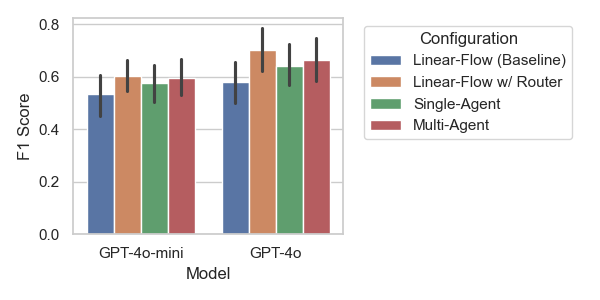
\includegraphics[width=0.7\textwidth]{images_exp2/bar_best_f1_by_model_and_configuration.png}
            \caption{Best F1-Score by model and configuration.}
            \label{fig:best_f1_by_model_and_configuration}
        \end{figure}

        The distribution of F1-scores, shown in the boxplot in Figure \ref{fig:f1_score_by_model_and_configuration}, further reinforces this finding. The Multi-Agent and Single-Agent configurations not only achieve higher median scores but also exhibit less variance compared to the Linear-Flow setups, indicating more consistent and reliable performance across the diverse set of questions.

        \begin{figure}[h]
            \centering
            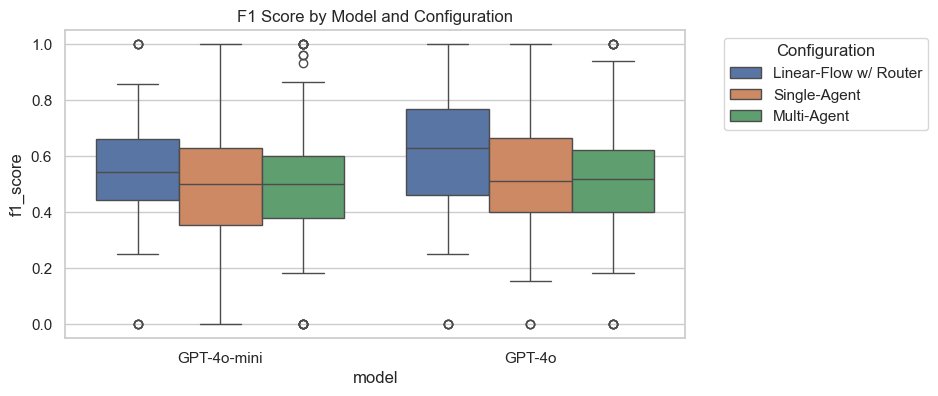
\includegraphics[width=0.9\textwidth]{images_exp2/f1_score_by_model_and_configuration.png}
            \caption{F1-Score distribution by model and agent configuration.}
            \label{fig:f1_score_by_model_and_configuration}
        \end{figure}

        In addition to the F1-scores, a more detailed breakdown of performance, including precision and recall, is presented in Table \ref{tab:performance_metrics}. These metrics provide a more granular view of each configuration's strengths and weaknesses.

        \begin{landscape}
            \begin{table}[H]
            \centering
            \caption{F1-Score, Precision and Recall statistics by model and configuration.}
            \label{tab:stats_by_model_config}
            % \resizebox{\textwidth}{!}{%
            \begin{tabular}{@{}llcccccccccccc@{}}
                \toprule
                \multirow{2}{*}{\textbf{Model}} & \multirow{2}{*}{\textbf{Configuration}} & \multicolumn{4}{c}{\textbf{F1-Score}} & \multicolumn{4}{c}{\textbf{Precision}} & \multicolumn{4}{c}{\textbf{Recall}} \\
                \cmidrule(l){3-6} \cmidrule(l){7-10} \cmidrule(l){11-14}
                & & Mean & Std. Dev. & Min & Max & Mean & Std. Dev. & Min & Max & Mean & Std. Dev. & Min & Max \\
                \midrule
                \multirow{4}{*}{GPT-4o} & Linear-Flow (Baseline) & 0.581 & 0.204 & 0.000 & 1.000 & 0.656 & 0.262 & 0.000 & 1.000 & 0.548 & 0.201 & 0.000 & 1.000 \\
                & Linear-Flow w/ Router & 0.702 & 0.202 & 0.333 & 1.000 & 0.805 & 0.185 & 0.400 & 1.000 & 0.674 & 0.242 & 0.286 & 1.000 \\
                & Multi-Agent & 0.664 & 0.214 & 0.286 & 1.000 & 0.746 & 0.221 & 0.286 & 1.000 & 0.630 & 0.231 & 0.286 & 1.000 \\
                & Single-Agent & 0.643 & 0.213 & 0.364 & 1.000 & 0.751 & 0.198 & 0.400 & 1.000 & 0.618 & 0.240 & 0.294 & 1.000 \\
                \midrule
                \multirow{4}{*}{GPT-4o-mini} & Linear-Flow (Baseline) & 0.534 & 0.208 & 0.000 & 0.923 & 0.604 & 0.262 & 0.000 & 1.000 & 0.516 & 0.216 & 0.000 & 0.923 \\
                & Linear-Flow w/ Router & 0.604 & 0.155 & 0.333 & 1.000 & 0.676 & 0.196 & 0.300 & 1.000 & 0.602 & 0.206 & 0.267 & 1.000 \\
                & Multi-Agent & 0.596 & 0.182 & 0.348 & 1.000 & 0.687 & 0.198 & 0.400 & 1.000 & 0.578 & 0.201 & 0.235 & 1.000 \\
                & Single-Agent & 0.576 & 0.184 & 0.308 & 1.000 & 0.719 & 0.214 & 0.286 & 1.000 & 0.544 & 0.227 & 0.231 & 1.000 \\
                \bottomrule
            \end{tabular}%
            % }
            \end{table}

        \end{landscape}













    \subsection{Discussion}

        The results of this second experimental cycle provide clearer insights into the effectiveness of different LLM architectures.
        \begin{itemize}
            \item \textbf{Agentic Architectures are Superior:} Both the Single-Agent and Multi-Agent Supervisor setups significantly outperformed the non-agentic Linear-Flow baselines. This demonstrates that for complex, multi-faceted questions requiring information from diverse sources, a simple "retrieve-then-read" RAG pipeline is insufficient. The iterative reasoning, planning, and tool-use capabilities inherent to agentic frameworks are crucial for achieving high performance.

            \item \textbf{Specialization and Collaboration Pay Off:} The Multi-Agent Supervisor architecture achieved the highest F1-score. This suggests that decomposing a complex problem and assigning sub-tasks to specialized agents is a highly effective strategy. The supervisor acts as a reasoning orchestrator, leveraging the focused expertise of each team member, which leads to more comprehensive and accurate answers.

            \item \textbf{Model Capability Matters:} Across all architectures, the GPT-4 model consistently outperformed GPT-3.5-turbo. This is particularly evident in the more complex agentic setups, where the superior reasoning and instruction-following capabilities of the more advanced model can be fully leveraged.

            \item \textbf{Limitations and Future Work:} While the automated evaluation methodology proved scalable and objective, it has its own limitations. The LLM-as-a-Judge is not infallible and can be influenced by its own internal biases or the phrasing of the evaluation prompt. Furthermore, the ground-truth answers, while expert-validated, represent just one possible correct response. Future work could explore ensemble judging methods to increase evaluation reliability and investigate more advanced agentic structures, such as those that allow for dynamic team formation or incorporate self-correction loops.
        \end{itemize}

        In summary, this second, more rigorous experimental cycle confirms that for complex, domain-specific tasks, sophisticated agentic architectures like a Multi-Agent Supervisor provide the best performance. Their ability to decompose problems and orchestrate specialized agents leads to more precise and complete answers than either non-agentic pipelines or monolithic single-agent systems.

        
        [TODO: FURTHER RESULTS WILL BE ADDED HERE]